\documentclass[../main.tex]{subfiles}

\graphicspath{{../images/}}

\begin{document}
\pagestyle{fancy}
\lhead{Module 2}
\chead{Junseo Shin}
\rhead{CSE 4059}

\section{Module 2}

\subsection*{DeviceQuery}

\begin{figure}
    [ht]
    \centering
    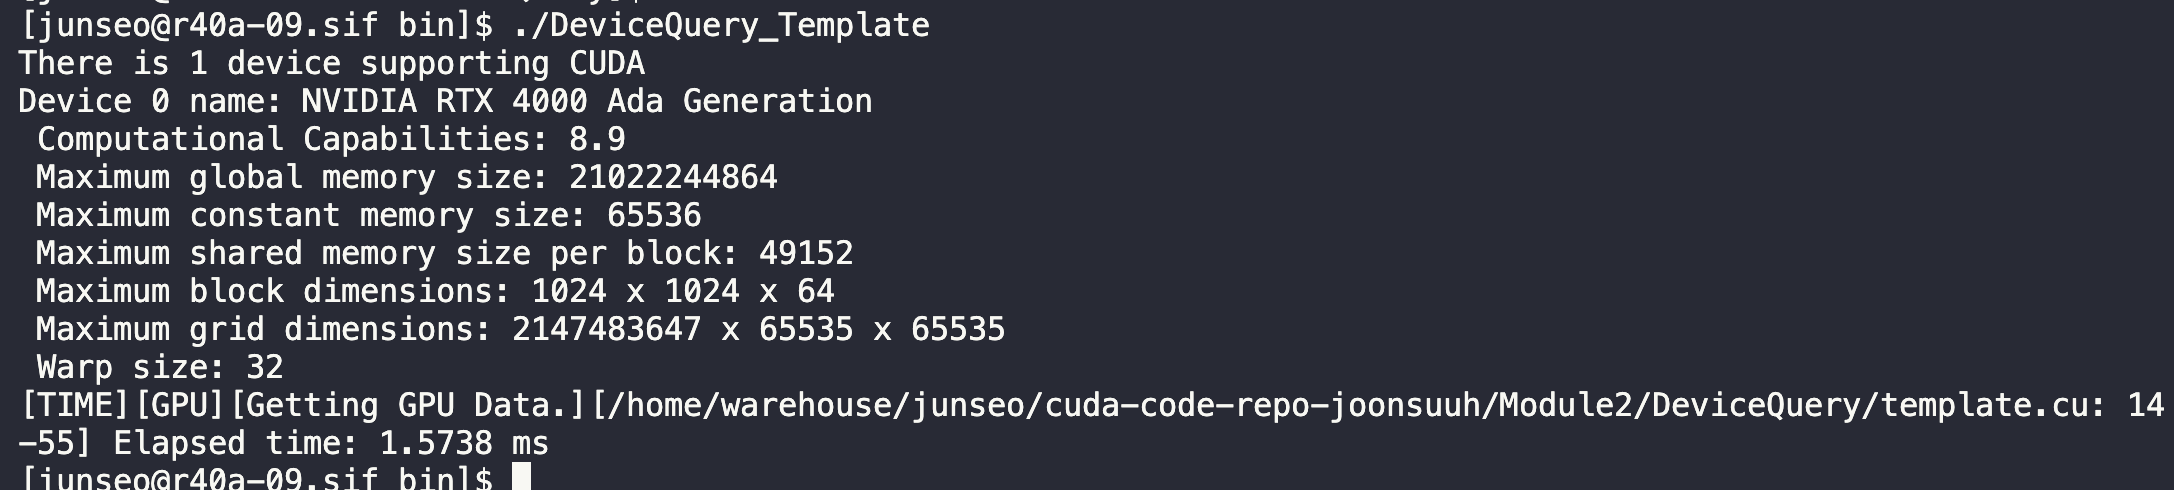
\includegraphics[width=0.8\textwidth]{devicequery.png}
    \caption{\texttt{DeviceQuery\_template} output}
\end{figure}

\subsection*{Questions}

\begin{enumerate}
    \item What is the compute capability of the NVIDIA Ada architecture?

    Compute Capability: 8.9

    \item What are the maximum block dimensions for GPUs with the compute
    capability of this architecture?

    Max block dimensions: $1024 \times 1024 \times 64$

    \item Suppose you are launching a one dimensional grid and block. If the
    hardware’s maximum grid dimension is 65535 and the maximum block
    dimension is 1024, what is the maximum number threads can be launched
    on the GPU?

    Max number of threads: $65535 \times 1024 = 67107840$

    \item Under what conditions might a programmer choose not want to launch
    the maximum number of threads?

    If multiple kernels are launched at the same time, then a programmer shouldn't launch
    the maximum number of threads on each kernel function.

    \item What can limit a program from launching the maximum number of threads
    on a GPU?

    The memory capacity of the GPU can limit a program from launching the
    maximum number of threads---e.g, if 

    \item What is shared memory?
    
    The memory allocated to thread blocks that can be accessed by all threads in the block which
    allows for low latency access to the data per SM (Streaming Multiprocessor).

    \item What is global memory?
    
    Memory that is visiable to all thread blocks and specified by the DRAM of the device
    (GPU)---e.g. a GeForce RTX 4090 has 24 GB of GDDR6X global
    memory---allocated using \texttt{cudaMalloc()} or
    \texttt{cudaMallocManaged()} for CUDA API.

    \item What is constant memory?
    
    Similar to global memory i.e. visible to all thread blocks, but is read-only and can't be
    changed by the threads on the device kernel function.

    \item What does warp size signify on a GPU?
    
    It is the number of threads in a block that are assigned/partitioned to an SM. For example, the warp size
    of the NVIDIA Ada architecture is 32 threads. E.g. 
    
    \begin{itemize}
        \item A one-dimensional block with 64 threads will be partitioned into 2 warps.
    \end{itemize}
\end{enumerate}




\end{document}